\section{Zadání}

Seznamte se s jádrem datového modelu IS STAG a vytvořte v nástroji Oracle Data Integrator Studio integrační projekt.
Předpokládá se, že výsledný projekt bude integrovat data do výsledného modelu obsahující minimálně dvě tabulky v relaci 1:N.
Bylo by též vhodné, aby nad jednou z těchto tabulek byla provedena vhodná selekce a druhá tabulka získala novou hodnotu za pomoci agregované funkce.

Téma: Průměrné hodnocení Diplomových prací z kateder FAV,

\begin{itemize}
    \item filtrace: katedry FAV (dimenzionální tabulka);
    \item agregace: průměrné hodnocení DP z kateder (faktová tabulka agregovaná přes obory).
\end{itemize}

\section{Analýza}
Cílem naší semestrální práce bylo zjistit průměrné hodnocení diplomových prací v rámci jednotlivých kateder na Fakultě aplikovaných věd. Abychom tento úkol mohli realizovat, museli jsme nejprve vybrat vhodné tabulky z demo databáze stagu. Stag obsahuje více než 400 tabulek, z čehož jen jeho jádro tvoří více než 50 z nich. Zorientování se v databázi bylo velmi náročné. 

Po analýze obsahu tabulek stagu, jsme pro náš vstupní model vybrali tabulky \textit{OBORY}, \textit{CIS\_PRACOVIST} a \textit{ABN\_DIPLOMOVE\_PRACE}. 

Nejjednodušší z nich je tabulka \textit{CIS\_PRACOVIST}, která představuje číselník pracovišť na ZČU.
Tabulka obsahuje 19 různých atributů.
Pro nás jsou však důležité pouze první tři a to \textit{ZKR} (zkratka pracoviště, datový typ VARCHAR2(6 BYTE)), \textit{NAZEV} (název pracoviště, datový typ VARCHAR2(100 BYTE)) a \textit{CISLO\_PRAC} (číslo pracoviště, datový typ VARCHAR2(16 BYTE) ).
Primární klíč tabulky tvoří sloupec \textit{ZKR}.
Tuto tabulku jsme použili pro získání názvů kateder na FAV (více viz sekce Mapování). 

Tabulka \textit{OBORY} reprezentuje seznam oborů vyučovaných na ZČU.
Relevantní sloupce pro naši úlohu jsou sloupce \textit{OBORIDNO} (ID oboru, datový typ NUMBER(10,0)), \textit{CZ\_NAZEV} (název oboru, datový typ VARCHAR2(200 BYTE)), \textit{ZKR} (zkratka oboru, datový typ VARCHAR2(10 BYTE)), \textit{PRAC\_ZKR} (zkratka pracoviště, datový typ VARCHAR2(6 BYTE)) a \textit{FAKULTA\_OBORU} (fakulta oboru, datový typ VARCHAR2(6 BYTE)). Primární klíč tvoří sloupec \textit{OBORNO}. Tuto tabulku jsme využili pro získání oborů vyučovaných na FAV. 

Poslední a nejdůležitější vybranou tabulkou je tabulka \textit{ABN\_DIPLOMOVE\_PRACE}. 
Z této tabulky jsme využili sloupce \textit{ZNAMKA} (výsledná známka DP, datový typ NUMBER(2,1)),  \textit{PRAC\_ZKR} (zkratka pracoviště, datový typ VARCHAR2(6 BYTE)) a \textit{OBORIDNO} (klíč do tabulky Obory, datový typ NUMBER(10,0)). Tuto tabulku jsme využili pro získání známek diplomových prací. 

Tyto tabulky tvoří náš vstupní model. Vztahy mezi tabulkami ukazuje obr. č. \ref{fig:src-model}. 

\begin{figure}[htb]
    \centering
    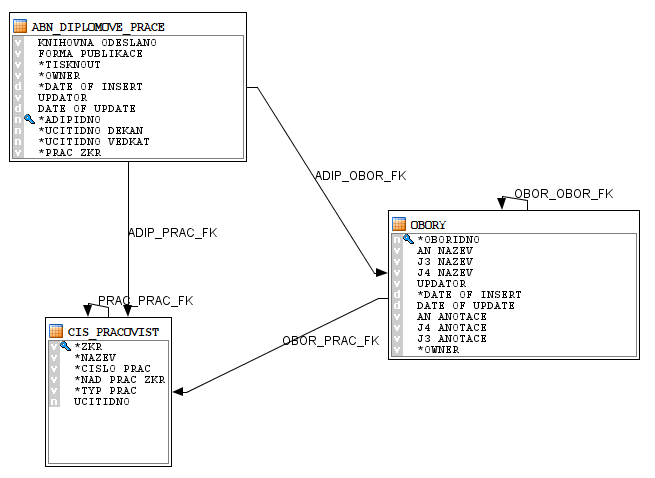
\includegraphics[width=0.7\textwidth]{graphs/src-model.png}
    \caption{Vstupní model}
    \label{fig:src-model}
\end{figure}
\FloatBarrier

\section{Vypracování}

\subsection{Datové zdroje a schémata}

Proces vypracování úkolu se skládal z několika kroků.
Předpokladem pro vytvoření komponent ETL bylo založení hlavního (MASTER\_INS\_REPO) a~pracovního repozitáře (TAUCHENL\_REPO).
Tyto dva repozitáře jsme již měli založené z jednoho z prvních cvičení předmětu.
Věnovali jsme se tedy rovnou založení datových zdrojů.

Datové zdroje jsme pro náš projekt potřebovali dva - jeden pro zdrojovou databázi \textit{LOVCIM\_ZDROJ3} a jeden pro cílovou databázi \textit{LOVCIM\_CIL}.
Druhý zmíněný datový zdroj jsme taktéž měli založený již z dřívějška.

Dalším krokem bylo vytvořit fyzické a logické schéma.
Fyzické schéma datového modelu reprezentuje strukturu databáze na fyzické úrovni.
Jde o popis vlastního uložení dat (např. uložení záznamu o konkrétním studentovi).
Fyzické schéma pro zdrojovou databázi se v našem případě jmenuje \textit{LOVCIM\_ZDROJ3.INSTALL2} a používá schéma účtu INSTALL2 a pracovní schéma účtu LOFFEL.
Toto nastavení souvisí s přiřazením různých uživatelských rolí a příslušných práv pro přístup k datům používané demo databáze stagu.
Účet \textit{INSTALL2} je specifickým účtem, který obsahuje všechny tabulky databáze.
Účet \textit{LOFFEL} je jedním z administrátorských účtů, který jako takový má přístup ke všem tabulkám. 

Logické schéma reprezentuje logickou strukturu databáze.
Jinak řečeno, logické schéma popisuje, jaká data jsou v databázi uložena a jaké jsou vztahy mezi těmito daty.
Logické schéma v ODI Studiu kombinuje dvojici kontext (viz dále) a fyzické schéma, které tímto logickým schématem svážeme dohromady.
V naší úloze bylo potřeba založit opět pouze jedno schéma - logické schéma pro zdrojovou databázi(\textit{Zdrojova\_databaze\_SP}).
Logické schéma pro cílovou databázi už v projektu existovalo.

Ke správnému nastavení obou schémat byl zapotřebí výše zmíněný kontext.
Kontext je množina prostředků umožňujících provoz nebo simulaci jedné nebo více aplikací, které zpracovávají data.
Do naší úlohy jsme využili již existující kontext \textit{lovcim}, který jsme nastavili u obou nově vytvořených schémat. 

Konečný stav vytvořených datových zdrojů a schémat je uveden v tabulce~\ref{table:table3}.

\begin{table}[htb]
    \centering

    \begin{tabular}{lll}
        \toprule

                        & Zdroj                     & Cíl                   \\ \midrule
        Datový zdroj    & LOVCIM\_ZDROJ3            & LOVCIM\_CIL           \\
        Fyzické schéma  & LOVCIM\_ZDROJ3.INSTALL2   & LOVCIM\_CIL.LOVCIM    \\
        Schéma          & INSTALL2                  & LOVCIM                \\
        Pracovní schéma & LOFFEL                    & LOVCIM                \\
        Logické schéma  & Zdrojova\_databaze\_SP    & Cilova\_databaze      \\
        Kontext         & lovcim                    & lovcim                \\
          
        \bottomrule
    \end{tabular}

    \caption{Konečný stav vstupních a výstupních zdrojů \& schémat}
    \label{table:table3}
\end{table}
\FloatBarrier

\subsection{Datové modelování}

Po připravení datových zdrojů jsme mohli začít s datovým modelováním.
Založili jsme dva datové modely.
Prvním datovým modelem je model \textit{Diplomky}.
Jde o model zdrojový, ze kterého se načítají data při mapování.
Tento datový model se skládá ze 3 tabulek: 

\begin{itemize}
    \item ABN\_DIPLOMOVE\_PRACE: tabulka obsahující data o diplomových pracích,
    \item CIS\_PRACOVIST: číselník pracovišť ZČU,
    \item OBORY: tabulka obsahující data o oborech na ZČU.
\end{itemize}

Jak již bylo řečeno, tyto tabulky jsou zdrojové a jsou obsaženy ve zdrojové databázi demo stagu, odkud bylo potřeba je načíst.
Vybrané tabulky vč. dat jsme načetli pomocí reverzního inženýrství.
Vztahy mezi načtenými tabulkami jsou vidět na obrázku číslo~\ref{fig:src-model}.

Tabulky obsahují i pro náš úkol nepotřebná data (= nepotřebné sloupce).
Ty je možné v Odi studiu z tabulek odebrat přes menu pro příslušný datový model.
Přesněji řečeno postupem: \textbf{Designer} -> \textbf{Models} -> \textbf{<Model folder>} -> \textbf{<Model>} -> \textbf{<Tabulka>} (pravý klik) -> \textbf{Open} -> \textbf{Attributes}.
Po výběru nepotřebných atributů je možné sloupce z modelu pomocí tlačítka \textit{Delete Attribute} odstranit. 

Druhým modelem je výstupní model \textit{Diplomky\_vystup}.
Do tohoto modelu jsou uloženy výsledky z mapování.
Na rozdíl od zdrojového modelu, ve kterém stačilo pouze načíst již existující tabulky, zde jsme museli nejprve cílové tabulky ve výstupním datovém zdroji založit.

Pro založení výstupních tabulek jsme použili skript, který je vidět níže v sekci Zakládací skript.
Pomocí tohoto skriptu jsme založili tabulky \textit{TRG\_KATEDRY} a \textit{TRG\_HODNOCENI\_DP}.
Do modelu \textit{Diplomky\_vystup} jsme je načetli opět reverzním inženýrstvím.  

\subsection{Zakládací skript}

\begin{lstlisting}[language=sql]

CREATE TABLE TRG_KATEDRY (
  KATEDRA_ID NUMERIC(16),
  KATEDRA_KOD VARCHAR(50) NOT NULL,
  KATEDRA_NAZEV VARCHAR(100),

  CONSTRAINT PK_TRG_KATEDRY PRIMARY KEY (KATEDRA_KOD)
);

CREATE TABLE TRG_HODNOCENI_DP (
  KATEDRA_KOD VARCHAR(50),
  OBOR_ID NUMERIC(10) NOT NULL,
  OBOR_NAZEV VARCHAR(55),
  HODNOCENI VARCHAR(50),

  CONSTRAINT PK_TRG_HODNOCENI_DP PRIMARY KEY (OBOR_ID),
  CONSTRAINT FK_KATEDRY_HONOCENI FOREIGN KEY (KATEDRA_KOD) REFERENCES TRG_KATEDRY (KATEDRA_KOD)
);
\end{lstlisting}

\subsection{Mapování}

Posledním krokem vypracování úkolu bylo samotné mapování.
Máme dvě výstupní tabulky, proto mějme 2 mapovací procedury.

První mapování slouží k výrobě dimenzionální tabulky obsahující katedry FAV.
Filtrem na sloupec \textit{OBORY.FAKULTA\_OBORU} (=\'FAV\') vybereme pouze obory patřící pod FAV, vyfiltrovanou tabulku dále napojíme (join) na číselník pracovišť (\textit{OBORY.PRAC\_ZKR = CIS\_PRACOVIST.ZKR}).
Z číselníku pracovišť vybereme název katedry a její číselný kód.
Prvkem \textit{DISTINCT\_} se pak vyvarujeme případným nekonzistencím v datech demo databáze.

\begin{figure}[htb]
    \centering
    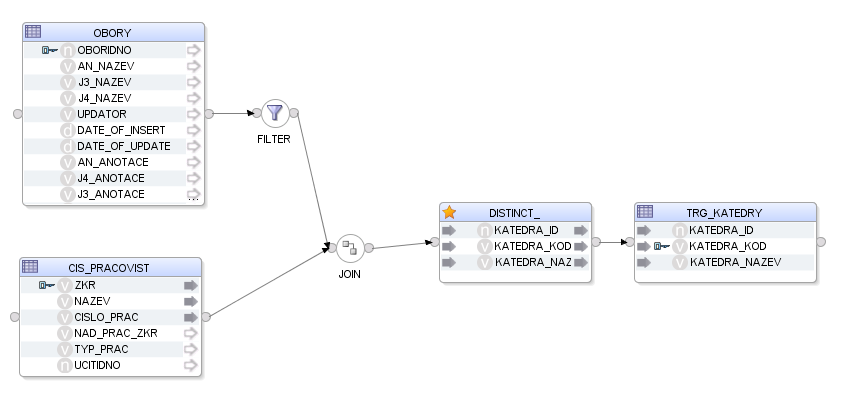
\includegraphics[width=0.7\textwidth]{graphs/odi-mapping-trg-katedry.png}
    \caption{ODI Výstupní mapování do tabulky TRG\_KATEDRY, logické schéma}
    \label{fig:odi-mapping-trg-katedry}
\end{figure}
\FloatBarrier

\begin{figure}[htb]
    \centering
    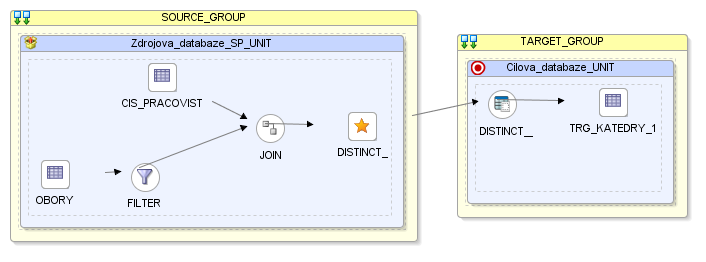
\includegraphics[width=0.7\textwidth]{graphs/odi-mapping-trg-katedry-physical.png}
    \caption{ODI Výstupní mapování do tabulky TRG\_KATEDRY, fyzické schéma}
    \label{fig:odi-mapping-trg-katedry-physical}
\end{figure}
\FloatBarrier

Obdobně postupujeme v případě druhého mapování.
Vyfiltrujeme pouze obory FAV, napojíme tabulku s hodnocením diplomových prací (\textit{ABN\_DIPLOMOVE\_PRACE.OBORIDNO = OBORY.OBORIDNO}).
Ze cvičných důvodů napojíme i číselník pracovišť (\textit{CIS\_PRACOVIST.ZKR = OBORY.PRAC\_ZKR}).
V zadání jsme definovali, že faktová tabulka bude obsahovat agregované hodnoty přes obory.
Vlastnosti bloku AGGREGATE jsou v tabulce~\ref{table:table4}.

\begin{table}[htb]
    \centering

    \begin{tabular}{ll}
        \toprule

        Atribut         & Výraz                             \\ \midrule
        KATEDRA\_KOD    & CIS\_PRACOVIST.ZKR                \\
        OBOR\_ID        & OBORY.OBORIDNO                    \\
        OBOR\_NAZEV     & OBORY.CZ\_NAZEV                   \\
        HODNOCENI       & AVG(ABN\_DIPLOMOVE\_PRACE.ZNAMKA) \\
          
        \bottomrule
    \end{tabular}

    \caption{Vlastnosti bloku aggregate}
    \label{table:table4}
\end{table}
\FloatBarrier

\begin{figure}[htb]
    \centering
    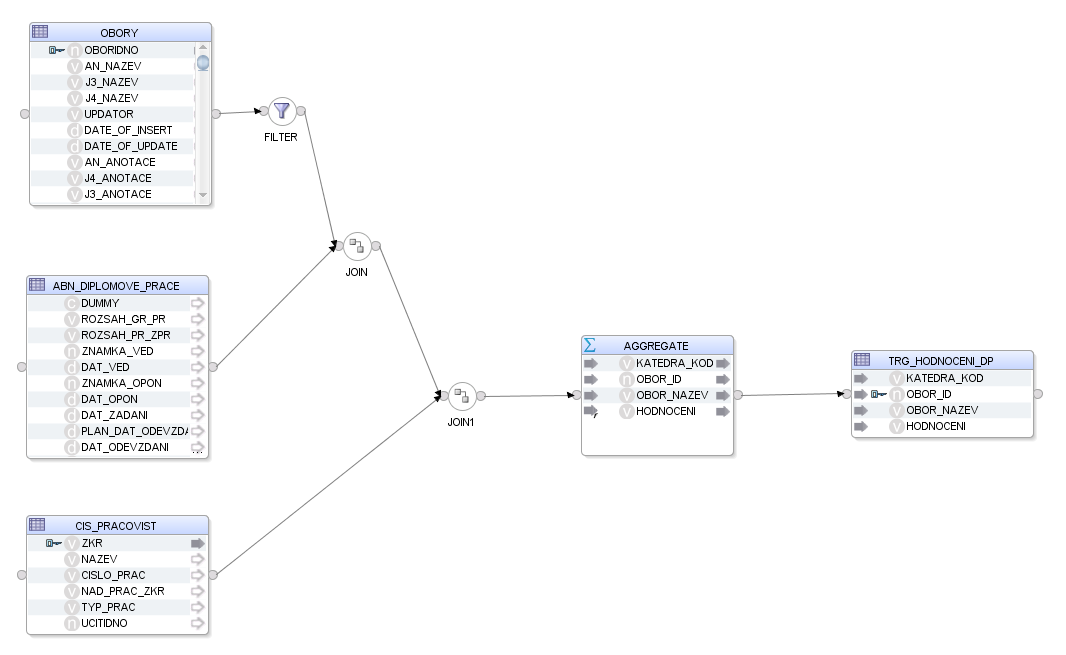
\includegraphics[width=0.7\textwidth]{graphs/odi-mapping-trg-hodnoceni-dp.png}
    \caption{ODI Výstupní mapování do tabulky TRG\_HODNOCENI\_DP, logické schéma}
    \label{fig:odi-mapping-trg-hodnoceni}
\end{figure}
\FloatBarrier

\begin{figure}[htb]
    \centering
    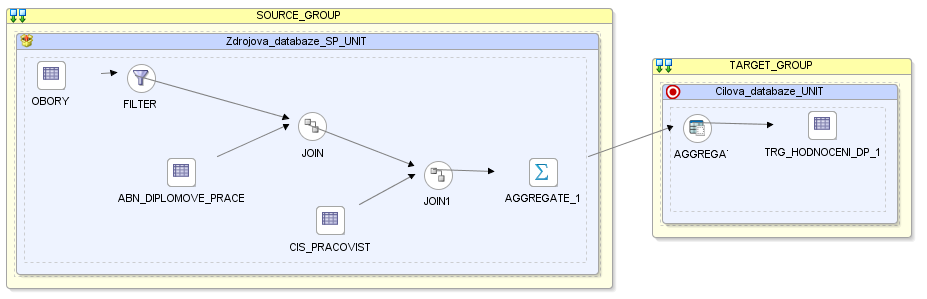
\includegraphics[width=0.7\textwidth]{graphs/odi-mapping-trg-hodnoceni-dp-physical.png}
    \caption{ODI Výstupní mapování do tabulky TRG\_HODNOCENI\_DP, fyzické schéma}
    \label{fig:odi-mapping-trg-hodnoceni-physical}
\end{figure}
\FloatBarrier

Poslední obrázek ukazuje nabídku transformačních komponent ODI Studia.

\begin{figure}[htb]
    \centering
    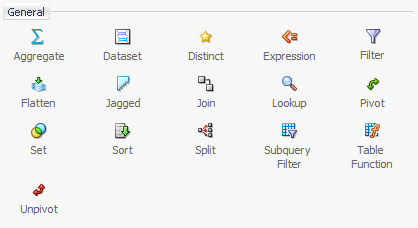
\includegraphics[width=0.55\textwidth]{graphs/odi-transformation-components.png}
    \caption{ODI nabídka komponent}
    \label{fig:odi-transformation-components}
\end{figure}
\FloatBarrier

\subsection{Výstupní model \& data}

Model výstupních dat je znázorněn na obrázku~\ref{fig:trg-model}.
Myšlenka tohoto schéma je poskytnout dimenzionální pohled na data, s tabulkou \textit{TRG\_KATEDRY} jako dimenzí a \textit{TRG\_HODNOCENI\_DP} jako faktovou tabulkou.

\begin{figure}[htb]
    \centering
    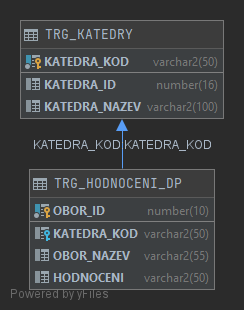
\includegraphics[width=0.3\textwidth]{graphs/trg-model.png}
    \caption{Výstupní model}
    \label{fig:trg-model}
\end{figure}
\FloatBarrier

Výstupní data z transformací jsou k vidění v tabulkách~\ref{table:table1}~\&~\ref{table:table2}.
Jak již vyplývá z předešlého popisu, tabulka \textit{Katedry} obsahuje 3 sloupce: \textit{KATEDRA\_ID}, \textit{KATEDRA\_KOD} a \textit{KATEDRA\_NAZEV}.

\textit{KATEDRA\_ID} měl původně sloužit jako primární klíč celé tabulky, z důvodu praktičnosti byl však v účelu nahrazen jejím kódem.
Tabulka obsahuje, dle zadání, pouze katedry FAV.

\begin{table}[htb]
    \centering

    \begin{tabular}{lll}
        \toprule

        KATEDRA\_ID & KATEDRA\_KOD  & KATEDRA\_NAZEV                            \\ \midrule
        52110       & KFY           & Katedra fyziky                            \\
        52120       & KME           & Katedra mechaniky                         \\
        52130       & KMA           & Katedra matematiky                        \\
        52140       & KKY           & Katedra kybernetiky                       \\
        52150       & KIV           & Katedra informatiky a výpočetní techniky  \\
        52160       & KGM           & Katedra geomatiky                         \\
          
        \bottomrule
    \end{tabular}

    \caption{Data ve výstupní tabulce TRG\_KATEDRY}
    \label{table:table1}
\end{table}
\FloatBarrier

Faktová tabulka \textit{Hodnocení} obsahuje 4 sloupce: \textit{KATEDRA\_KOD}, \textit{OBOR\_ID}, \textit{OBOR\_NAZEV} a~\textit{HODNOCENI}.
Abychom docílili splnění zadání, hodnocení je agregát (průměrná hodnota) hodnocení pro každý z oborů referencovaných kateder.
Jelikož by každý obor měl být v tabulce pouze jednou, je identifikační číslo oboru použito jako primární klíč.

\begin{table}[htb]
    \centering

    \begin{tabular}{llll}
        \toprule

        KATEDRA\_KOD    & OBOR\_ID  & OBOR\_NAZEV                       & HODNOCENI \\ \midrule
        KIV             & 2252      & Softwarové inženýrství            & 2,25      \\
        KGM             & 2309      & Geomatika                         & 4         \\
        KGM             & 2358      & Geomatika                         & 1,875     \\
        KKY             & 3808      & Automatické řízení a robotika     & NULL      \\
        KMA             & 2130      & Finanční informatika a statistika & 2,6667    \\
        \ldots          & \ldots    & \ldots                            & \ldots    \\

        \bottomrule
    \end{tabular}

    \caption{Ukázková data z výstupní tabulky TRG\_HODNOCENI\_DP}
    \label{table:table2}
\end{table}
\FloatBarrier

V tabulce si můžeme povšimnout, že např. obor \textit{Geomatika} se objevuje dvakrát, s odlišným ID.
To bude způsobeno reálností dat.
Předpokládáme totiž, že při nové atestaci stejného oboru se zachová jeho název, změní se však jeho ID.

Dalším zajímavým jevem je výskyt průměrného hodnocení 4, a přítomnosti NULL hodnoty.
To je zase způsobeno nedostatečnou reálností testovacích dat, kdy vygenerovaní studenti a diplomové práce nebudou dostatečně pokrývat prostor dat.
Po kontrolním výběru dat jsme zjistili, že v obou případech (případ průměrného hodnocení 4 a NULL) je oboru přiřazena právě jedna diplomová práce, po jedné s hodnocením 4 a bez hodnocení.

\section{Závěr}

V semestrální práci jsme si vyzkoušeli proces vytváření datové transformace.
Tento proces byl náplní praktických cvičení, jednalo se tedy hlavně o důkaz replikovatelnosti postupu na vlastním zadání.
Použitý nástroj, Oracle Data Integrator, je jeden z nejrozšířenějších ETL produktů vůbec.

Praktická cvičení a semestrální práce nám tedy poskytly cennou příležitost zkusit si s tímto nástrojem pracovat a řešit případné potíže, které mohou při konstrukci transformací nastat.
V našem konkrétním případě se pak jedná i o zajímavé propojení předmětů, jelikož jsme zvolili transformaci z logického databázového modelu do dimenzionální struktury, poskytujíc referenci na předmět KIV/DBM2.

Jelikož nástroj ODI není jediným produktem tohoto zaměření, stojí za to zmínit silné a slabé stránky produktu.
Společnost Oracle je velmi silný dodavatel, poskytující robustní podporu svých produktů, a to zejména v případech tak ověřených nástrojů jakým je Data Integrator.
Na druhou stranu nelze opomenout zastaralé uživatelské rozhraní, strmou křivku učení a v našich podmínkách velmi pomalé chování.

Za zmínku stojí také možnost nahlédnutí do databáze demo verze systému IS STAG, která přes přítomnost pouze testovacích dat poskytuje bohaté datové schéma k prozkoumání.
